\documentclass[11pt]{article}
\usepackage[margin=1in]{geometry}
\usepackage{amsmath,amssymb,amsthm}
\usepackage{booktabs}
\usepackage{graphicx}
\usepackage{tikz}
\usetikzlibrary{calc,arrows.meta,positioning,decorations.pathreplacing,fit}

\newtheorem{theorem}{Theorem}[section]
\newtheorem{lemma}[theorem]{Lemma}
\newtheorem{proposition}[theorem]{Proposition}
\newtheorem{corollary}[theorem]{Corollary}
\theoremstyle{remark}
\newtheorem{remark}[theorem]{Remark}

% Fake labels from earlier sections
\newcommand{\fakeref}[1]{??}

% Stub citations
\newcommand{\nocitex}[1]{}

% Override \cite to not fail
\usepackage{cite}

% Fake earlier labels
\makeatletter
\newcommand\fakelabel[1]{\@bsphack\protected@write\@auxout{}{\string\newlabel{#1}{{}{}}}\@esphack}
\makeatother

\begin{document}
\fakelabel{sec:lattice}
\fakelabel{sec:lattice-rmatrix}
\fakelabel{sec:lattice-extensions}
\fakelabel{sec:groupoid}
\fakelabel{sec:groupoid-bn}
\fakelabel{sec:groupoid-hierarchy}
\fakelabel{eq:ybe}
\fakelabel{eq:transfer-commute}
\setcounter{section}{4}

% Suppress citation warnings for test
\bibliographystyle{plain}

%% Section 5: The Categorical Phase Diagram
%% To be \input{} into the main document.

\section{The Categorical Phase Diagram}
\label{sec:hierarchy}

The three-level hierarchy of Section~\ref{sec:groupoid-hierarchy}
--- solvable, quasi-solvable, combinatorial --- is a classification
of R-matrices by how much of the Yang-Baxter equation they satisfy.
This section reveals what the hierarchy \emph{is}: three types of
monoidal category, three symmetry groups, three character theories,
governed by a single transition algebra.  The passage between levels
is not a loss of structure but a forgetting of structure --- precise,
irreversible, and mathematically natural.  What emerges is a phase
diagram in which the multiplicity of combinatorial models for LR
coefficients is not an accident of history but a necessary consequence
of the layered categorical architecture.


\subsection{Three types of monoidal categories}
\label{sec:hierarchy-monoidal}

The three levels of integrability correspond to three ways of equipping
a monoidal category with a notion of ``swapping'' two objects.
Each carries a different symmetry group, and the inclusions between
them are strict.

\subsubsection*{Symmetric monoidal categories}

The simplest structure is a \emph{symmetric monoidal category}: a
monoidal category equipped with a natural isomorphism
$\sigma_{V,W} \colon V \otimes W \xrightarrow{\sim} W \otimes V$
satisfying $\sigma_{W,V} \circ \sigma_{V,W} = \mathrm{id}_{V \otimes W}$.
The swap squares to the identity.  The prototypical example is
$\mathrm{Vect}$, the category of finite-dimensional vector spaces
with the usual transposition $v \otimes w \mapsto w \otimes v$.  The
symmetry group governing $n$-fold tensor products is the symmetric
group $S_n$: each permutation $\pi \in S_n$ acts on $V^{\otimes n}$
by permuting tensor factors, and the relation $\sigma^2 = \mathrm{id}$
ensures that the action factors through $S_n$.

\subsubsection*{Braided monoidal categories}

A \emph{braided monoidal category} is a monoidal category with a
natural isomorphism $\beta_{V,W} \colon V \otimes W \xrightarrow{\sim}
W \otimes V$ satisfying the \emph{hexagon axioms}, which encode the
Yang-Baxter equation categorically:
\begin{equation}
\label{eq:braid-ybe}
  (\beta_{V,W} \otimes \mathrm{id}_U) \circ
  (\mathrm{id}_V \otimes \beta_{U,W}^{-1})^{-1} \circ
  (\beta_{U,V} \otimes \mathrm{id}_W)
  \;=\;
  (\mathrm{id}_W \otimes \beta_{U,V}) \circ
  (\beta_{U,W} \otimes \mathrm{id}_V)^{-1} \circ \cdots
\end{equation}
but \emph{not} the involution $\beta^2 = \mathrm{id}$.  More
concretely: on a triple tensor product $U \otimes V \otimes W$,
writing $\beta_{12}$ for the braiding applied to the first two factors
and $\beta_{23}$ for the braiding on the last two, the hexagon axioms
reduce to
\begin{equation}
\label{eq:braid-relation}
  \beta_{12} \circ \beta_{23} \circ \beta_{12}
  \;=\;
  \beta_{23} \circ \beta_{12} \circ \beta_{23},
\end{equation}
the braid relation.  The symmetry group is the braid group $B_n$,
whose generators $\sigma_1, \ldots, \sigma_{n-1}$
satisfy~\eqref{eq:braid-relation} but are \emph{not} involutions.
The central example is $\mathrm{Rep}(U_q(\mathfrak{g}))$ for generic
$q$: the braiding $\beta_{V,W} = P \circ R_{V,W}$ is constructed from
Drinfeld's universal R-matrix, and the fact that $R$ satisfies the
parametric YBE of Section~\ref{sec:lattice-rmatrix} is precisely the
braid relation~\eqref{eq:braid-relation} in categorical language.

\subsubsection*{Coboundary monoidal categories}

Between symmetric and braided lies a structure with no classical
analogue in physics: the \emph{coboundary monoidal category},
introduced by Drinfeld and developed in the representation-theoretic
context by Henriques and
Kamnitzer~\cite{henriques-kamnitzer-2006}.  A coboundary category
is a monoidal category with a natural isomorphism $\sigma_{V,W} \colon
V \otimes W \xrightarrow{\sim} W \otimes V$---called the
\emph{commutor}---satisfying three axioms:
\begin{enumerate}
\item[(C1)] \emph{Involution:} $\sigma_{W,V} \circ \sigma_{V,W} =
  \mathrm{id}$.  (Like a symmetric category, but unlike a braided one.)
\item[(C2)] \emph{Disjoint commutativity:} if the intervals $[i,j]$
  and $[k,l]$ are disjoint subsets of $\{1, \ldots, n\}$, then the
  commutors $\sigma_{[i,j]}$ and $\sigma_{[k,l]}$ commute.
\item[(C3)] \emph{Nesting:} if $[k,l] \subseteq [i,j]$, then
  $\sigma_{[i,j]} \circ \sigma_{[k,l]} \circ \sigma_{[i,j]} =
  \sigma_{[\sigma(k), \sigma(l)]}$, where $\sigma$ denotes the
  reversal of $[i,j]$.
\end{enumerate}
These are the defining relations of the \emph{cactus group} $J_n$
of Devadoss and
Henriques-Kamnitzer~\cite{henriques-kamnitzer-2006}.  The cactus
group is generated by elements $s_{[i,j]}$ for $1 \leq i < j \leq n$,
subject to (C1)--(C3).  It is an infinite group (unlike $S_n$), and
its structure is genuinely distinct from both the braid group and the
symmetric group: $J_n$ admits a surjection onto $S_n$ (map each
interval reversal $s_{[i,j]}$ to the corresponding permutation), but
this surjection does \emph{not} split.

\begin{remark}[Non-splitting of $J_3$]
\label{rem:cactus-nonsplit}
For $n = 3$, the surjection $J_3 \twoheadrightarrow S_3$ does not
admit a group-theoretic section.  One can verify this directly: $J_3$
is generated by $s_{[1,2]}$, $s_{[2,3]}$, and $s_{[1,3]}$, with
$s_{[1,2]}^2 = s_{[2,3]}^2 = s_{[1,3]}^2 = 1$ and the nesting
relation $s_{[1,3]} s_{[1,2]} s_{[1,3]} = s_{[2,3]}$.  Any section
$S_3 \to J_3$ would need to send the transpositions $(12)$ and $(23)$
to elements $a, b \in J_3$ satisfying $a^2 = b^2 = 1$ and
$aba = bab$ (the braid relation modulo $\sigma^2 = 1$).  But in $J_3$,
the products $s_{[1,2]} s_{[2,3]} s_{[1,2]}$ and
$s_{[2,3]} s_{[1,2]} s_{[2,3]}$ are \emph{not} equal: the nesting
relation (C3) is not the braid relation.  No choice of lifts
satisfies all the $S_3$ relations simultaneously.  The cactus group
is not a semidirect product; the coboundary level does not retract
onto the symmetric level.
\end{remark}

\noindent
The central example of a coboundary monoidal category is
$\mathrm{Crys}(\mathfrak{g})$, the category of Kashiwara crystal
bases~\cite{kashiwara-1990}.  The Henriques-Kamnitzer crystal
commutor $\sigma_{V,W}^{\mathrm{crys}}$ is constructed from the
Sch\"utzenberger involution on highest-weight crystals and extended
to tensor products via a recursive procedure involving connected
components of the tensor product crystal graph.

\subsubsection*{The hierarchy is strict}

The three types form a chain of strict inclusions:
\[
  \text{symmetric} \;\subsetneq\; \text{coboundary}
  \;\subsetneq\; \text{braided}.
\]
Every symmetric category is coboundary (the swap $\sigma$ satisfies
the cactus relations trivially, since $\sigma^2 = 1$ and the nesting
relation collapses to a symmetric group identity).  Every coboundary
category can be \emph{embedded into} a braided one via the
Kamnitzer-Tingley unitarised R-matrix
construction~\cite{kamnitzer-tingley-2007} (see
Section~\ref{sec:hierarchy-hecke} below).  But neither inclusion
reverses: not every braided category admits a coboundary structure
(the braiding must be unitarisable), and not every coboundary category
is symmetric (the non-splitting of $J_3 \twoheadrightarrow S_3$ shows
the coboundary axioms are strictly weaker than the symmetric ones).

The three monoidal types correspond precisely to the three integrability
levels of Section~\ref{sec:groupoid-hierarchy}:
\begin{center}
\renewcommand{\arraystretch}{1.3}
\begin{tabular}{llll}
\toprule
\textbf{Monoidal type} & \textbf{Swap structure} & \textbf{Symmetry group}
  & \textbf{Integrability} \\
\midrule
Braided & $\beta^2 \neq \mathrm{id}$, braid relation &
  $B_n$ (braid) & Solvable \\
Coboundary & $\sigma^2 = \mathrm{id}$, cactus relations &
  $J_n$ (cactus) & Quasi-solvable \\
Symmetric & $\sigma^2 = \mathrm{id}$, braid = trivial &
  $S_n$ (symmetric) & Combinatorial \\
\bottomrule
\end{tabular}
\end{center}

\noindent
This alignment is the first axis of the phase diagram.  We now identify
what is forgotten at each transition.


\subsection{The Multiplicity Bundle Theorem}
\label{sec:hierarchy-multiplicity}

The passage from coboundary to symmetric is mediated by a single
geometric object: the \emph{multiplicity bundle}, whose fibre at each
isotypic component of a tensor product is the Specht module $S_\lambda$.
The coboundary commutor acts nontrivially on these fibres.  The crystal
functor kills them.  This is the content of the central theorem.

\subsubsection*{Setup}

Let $V = \mathbb{C}^n$ be the fundamental representation of
$GL_n(\mathbb{C})$, and let $k \geq 2$.  The Schur-Weyl decomposition
\begin{equation}
\label{eq:schur-weyl-2}
  V^{\otimes k} \;\cong\;
  \bigoplus_{\substack{\lambda \vdash k \\ \ell(\lambda) \leq n}}
  V_\lambda \otimes S_\lambda
\end{equation}
decomposes $V^{\otimes k}$ as a $(GL_n \times S_k)$-bimodule, with
$V_\lambda$ the irreducible $GL_n$-module and $S_\lambda$ the Specht
module for $S_k$.  We think of~\eqref{eq:schur-weyl-2} as a vector
bundle over the set of partitions $\lambda$: the ``base'' fibre is
$V_\lambda$ (the physical, or representation-theoretic, factor) and
the ``multiplicity'' fibre is $S_\lambda$ (the combinatorial factor
that records how many copies of $V_\lambda$ appear in the tensor
product).

For an interval $[i,j] \subseteq \{1, \ldots, k\}$, define the
\emph{interval reversal} $w_0^{[i,j]} \in S_k$ to be the longest
element of the parabolic subgroup $S_{\{i, i+1, \ldots, j\}}$: the
permutation that reverses the positions $i, i+1, \ldots, j$ and fixes
all others.  In particular, $w_0^{[1,k]}$ is the longest element of
$S_k$.  The interval reversal acts on $V^{\otimes k}$ by permuting
tensor factors: $w_0^{[i,j]}$ sends
$v_1 \otimes \cdots \otimes v_k$ to
$v_1 \otimes \cdots \otimes v_{i-1} \otimes v_j \otimes v_{j-1}
\otimes \cdots \otimes v_i \otimes v_{j+1} \otimes \cdots \otimes v_k$.

\begin{theorem}[Multiplicity Bundle]
\label{thm:multiplicity-bundle}
The coboundary commutor $\sigma_{[i,j]}$ on $V^{\otimes k}$
decomposes under~\eqref{eq:schur-weyl-2} as
\begin{equation}
\label{eq:mult-bundle}
  \sigma_{[i,j]} \;=\;
  \bigoplus_\lambda \bigl(\mathrm{id}_{V_\lambda} \otimes
  \rho_{S_\lambda}(w_0^{[i,j]})\bigr),
\end{equation}
where $\rho_{S_\lambda}$ denotes the Specht module representation of
$S_k$.
\end{theorem}

\begin{proof}[Proof sketch]
The commutor $\sigma_{[i,j]}$ is, by definition, the interval reversal
$w_0^{[i,j]}$ acting on $V^{\otimes k}$ by permutation of tensor
factors.  This action commutes with the diagonal $GL_n$-action (since
permuting tensor factors commutes with applying the same group element
to each factor).  By Schur's lemma, any $GL_n$-endomorphism of
$V^{\otimes k}$ decomposes as $\bigoplus_\lambda (\mathrm{id}_{V_\lambda}
\otimes \phi_\lambda)$ for some $\phi_\lambda \in \mathrm{End}(S_\lambda)$.
Since the commutor is precisely the action of $w_0^{[i,j]} \in S_k$,
and the Schur-Weyl decomposition identifies the $S_k$-action with
$\mathrm{id}_{V_\lambda} \otimes \rho_{S_\lambda}$, we obtain
$\phi_\lambda = \rho_{S_\lambda}(w_0^{[i,j]})$.
\end{proof}

\noindent
The theorem is essentially a corollary of Schur-Weyl duality.  Its
content lies not in the proof --- which is short --- but in the
\emph{interpretation}: the commutor lives entirely in the multiplicity
fibres $S_\lambda$.  It acts as the identity on the representation-theoretic
factor $V_\lambda$ and as the longest-element involution $\rho(w_0)$ on
the Specht module.

\subsubsection*{Crystal invisibility}

The crystal functor $\mathcal{F} \colon \mathrm{Rep}(GL_n) \to
\mathrm{Crys}(\mathfrak{sl}_n)$ sends a representation to its crystal
basis, retaining the combinatorial skeleton (weights, raising and
lowering operators) while forgetting the linear algebra.  On tensor
products of the fundamental representation, the crystal functor has a
decisive effect on the multiplicity bundle.

\begin{proposition}[Crystal multiplicity-freeness]
\label{prop:crystal-mf}
The tensor product crystal $B(\omega_1)^{\otimes k}$, where
$B(\omega_1)$ is the crystal of the fundamental representation of
$\mathfrak{sl}_n$ with $n \geq k$, is \emph{multiplicity-free}: each
connected component is isomorphic to a highest-weight crystal
$B(\lambda)$ for a distinct partition $\lambda \vdash k$.
\end{proposition}

\noindent
In the language of the multiplicity bundle: when $n \geq k$, each
fibre $S_\lambda$ is one-dimensional as a crystal (it contributes
exactly one copy of $B(\lambda)$).  The crystal functor replaces the
potentially large Specht module $S_\lambda$ with a single point.
Every endomorphism of a one-dimensional set is the identity.
Therefore:

\begin{corollary}[Crystal commutor is trivial]
\label{cor:crystal-trivial}
The crystal commutor $\mathcal{F}(\sigma_{[i,j]})$ is the identity on
$B(\omega_1)^{\otimes k}$ for $n \geq k$.  In particular, the crystal
category of fundamental representations is symmetric monoidal.
\end{corollary}

\noindent
This is the mechanism by which the coboundary structure becomes
invisible at the crystal level.  The commutor $\sigma_{[i,j]}$ acts
nontrivially --- the longest element $w_0$ is not the identity in
any Specht module of dimension greater than one --- but its action
is confined to fibres that the crystal functor collapses.  The Specht
module is the vessel that carries the coboundary structure; the crystal
functor drains it.

\begin{remark}
The restriction $n \geq k$ ensures multiplicity-freeness and hence
triviality of the crystal commutor on fundamental tensor products.
For general representations, the crystal commutor is nontrivial --- it
is the Henriques-Kamnitzer commutor, constructed from the
Sch\"utzenberger involution.  The general crystal category
$\mathrm{Crys}(\mathfrak{g})$ is coboundary monoidal, not symmetric.
The symmetric monoidal structure is a special feature of the
fundamental representations, where multiplicity-freeness makes the
coboundary commutor degenerate.  This is consistent with the fact that
the lattice models of Section~\ref{sec:lattice} use fundamental
representations (edge spins in $\{0,1\} = B(\omega_1)$): the
combinatorial level of the hierarchy lives in the multiplicity-free
regime.
\end{remark}

\subsubsection*{The two transitions}

Theorem~\ref{thm:multiplicity-bundle} identifies what is forgotten at
each step of the hierarchy:

\medskip
\noindent
\textbf{Braided $\to$ Coboundary: forget the spectral parameter.}
At generic $q$, the category $\mathrm{Rep}(U_q(\mathfrak{g}))$ carries
both a braiding $\beta_{V,W} = P \circ R_{V,W}$ (from the universal
R-matrix, depending on a spectral parameter $u$) and a coboundary
commutor $\sigma_{V,W}$ (from the unitarised R-matrix of Kamnitzer and
Tingley~\cite{kamnitzer-tingley-2007}).  These are \emph{different}
structures: $\beta$ satisfies the braid relation but $\beta^2 \neq
\mathrm{id}$; $\sigma$ is an involution satisfying the cactus relations
but not the braid relation.  At $q = 0$, the braiding dies --- the
R-matrix degenerates and the braid relation can no longer be formed ---
but the commutor $\sigma$ survives, because its construction uses only
the unitarised (eigenvalue-independent) part of the R-matrix.  The
passage from braided to coboundary is not a creation of new structure
but an \emph{extraction}: the coboundary commutor was always present,
and the specialisation $q = 0$ strips away the braided layer to
reveal it.

\medskip
\noindent
\textbf{Coboundary $\to$ Symmetric: forget the multiplicity bundle.}
The commutor $\sigma_{[i,j]} = \mathrm{id}_{V_\lambda} \otimes
\rho_{S_\lambda}(w_0^{[i,j]})$ acts nontrivially on $S_\lambda$
whenever $\dim S_\lambda > 1$.  The crystal functor kills $S_\lambda$
(Proposition~\ref{prop:crystal-mf}), collapsing the commutor to the
identity.  What was a rich action of the cactus group $J_n$ on
multiplicity spaces becomes the trivial action of $S_n$.

\medskip
\noindent
These two forgettings are irreversible.  The spectral parameter cannot
be recovered from the commutor (many braidings can produce the same
commutor via unitarisation).  The multiplicity bundle cannot be
recovered from the crystal (the crystal retains only the
$GL_n$-isotypic decomposition, not the $S_k$-module structure within
each isotypic component).  Each transition is a genuine loss of
information.


\subsection{The Hecke Transition Algebra}
\label{sec:hierarchy-hecke}

The three monoidal types are governed by a single algebraic object:
the Hecke algebra $H_q(S_k)$ and its degenerations.  The algebra
chain
\begin{equation}
\label{eq:hecke-chain}
  H_q(S_k) \;\xrightarrow{\;q \to 0\;}
  \; H_0(S_k) \;\xrightarrow{\;\text{semisimplify}\;}\;
  \mathbb{C}[S_k]
\end{equation}
mirrors the categorical hierarchy step by step.  The Hecke algebra is
not a fourth level of integrability; it is the \emph{algebra of the
transition itself}.

\begin{center}
\renewcommand{\arraystretch}{1.4}
\small
\begin{tabular}{llllll}
\toprule
\textbf{Level} & \textbf{Category type} & \textbf{Symmetry group}
  & \textbf{Fiber functor} & \textbf{YBE status} & \textbf{Characters} \\
\midrule
Solvable & Braided monoidal & $B_k$ (braid group)
  & $\Rep \to \Vect$ & Full YBE & Macdonald $P_\lambda$ \\
Quasi-solvable & Coboundary monoidal & $J_k$ (cactus group)
  & $\Rep \to \Crys$ & Column YBE & Key $\kappa_\alpha$ \\
Combinatorial & Symmetric monoidal & $S_k$ (symmetric group)
  & $\Crys \to \Set$ & None (trivial) & Schur $s_\lambda$ \\
\bottomrule
\end{tabular}
\end{center}

\subsubsection*{Generic $q$: the braided level}

At generic $q$, the Hecke algebra $H_q(S_k)$ is the quotient of the
group algebra of the braid group $B_k$ by the Hecke relation
$(T_i - q)(T_i + 1) = 0$.  The generators $T_1, \ldots, T_{k-1}$
satisfy the braid relation
\[
  T_i T_{i+1} T_i \;=\; T_{i+1} T_i T_{i+1}
\]
and the quadratic relation $T_i^2 = (q-1)T_i + q$.  In the lattice
model context of Section~\ref{sec:lattice}, the Hecke generator $T_i$
is the \emph{R-matrix} $\check{R}_i(u)$ acting on the $i$-th and
$(i+1)$-th tensor factors: the braid relation is the Yang-Baxter
equation, and the quadratic relation encodes the two nonzero eigenvalues
$q$ and $-1$ of the R-matrix.  The existence of two distinct eigenvalues
is what makes the braiding non-involutive ($\beta^2 \neq \mathrm{id}$)
and gives the braid group its infinite order.

The characters of $H_q$-modules, traced through the natural
representation on polynomial rings, yield the Macdonald polynomials
$P_\lambda(x; q, t)$ (at the most general level) and their
specialisations: Hall-Littlewood polynomials at $q = 0$, Schur
polynomials at $q = t$, and so on.  The solvable lattice models of
Section~\ref{sec:lattice} compute these characters as partition
functions.

\subsubsection*{$q = 0$: the coboundary level}

At $q = 0$, the Hecke relation becomes $T_i(T_i + 1) = 0$, or
equivalently $T_i^2 = -T_i$.  The Demazure operators
$\pi_i = T_i + 1$ satisfy
\begin{equation}
\label{eq:demazure-idem}
  \pi_i^2 = \pi_i,
\end{equation}
the idempotent relation.  This is the algebraic signature of the
coboundary level: the R-matrix has collapsed to a \emph{projector},
and the two eigenvalues $q$ and $-1$ have merged to $0$ and $-1$.
The braid relation among the $T_i$ persists formally, but it now
coexists with idempotency, and the combination produces the cactus
group rather than the braid group.

More precisely, define the cactus generators
\begin{equation}
\label{eq:cactus-from-hecke}
  \sigma_{[a,b]} \;=\; \pi_{w_0^{[a,b]}}
  \;=\; (T_{w_0^{[a,b]}} + 1)(T_{w_0^{[a,b]}} + 1) \cdots
\end{equation}
as the Demazure operator indexed by the longest element $w_0^{[a,b]}$
of the parabolic subgroup $S_{\{a, \ldots, b\}}$.  These operators
satisfy the cactus relations (C1)--(C3):
involution ($\sigma_{[a,b]}^2 = \mathrm{id}$ on suitable quotients),
disjoint commutativity, and nesting.  The verification is a direct
computation in $H_0$, confirmed numerically for $k \leq 5$.

Norton~\cite{norton-1979} showed that $H_0(S_k)$ has $2^{k-1}$ simple
modules, indexed by compositions $\alpha \models k$ rather than
partitions $\lambda \vdash k$.  The characters of these simple
modules are the \emph{Demazure atoms} $A_\alpha$: the nonsymmetric
polynomials from which key polynomials are built.  The key polynomial
$\kappa_\alpha$ is the character of the corresponding projective
indecomposable $H_0$-module, and the decomposition
\begin{equation}
\label{eq:key-schur}
  s_\lambda \;=\; \sum_{\alpha \sim \lambda} A_\alpha
\end{equation}
--- where the sum runs over compositions $\alpha$ that rearrange to
$\lambda$ --- is the character-level shadow of the semisimplification
$H_0 \to \mathbb{C}[S_k]$.

\subsubsection*{Semisimplification: the symmetric level}

The group algebra $\mathbb{C}[S_k]$ is the semisimplification of
$H_0(S_k)$: it identifies all compositions rearranging to the same
partition.  At the character level, this identification
is~\eqref{eq:key-schur}: the Schur polynomial is the sum of Demazure
atoms over compositions in the same $S_k$-orbit.  At the module level,
the $2^{k-1}$ simple $H_0$-modules (indexed by compositions) collapse
to the $p(k)$ simple $\mathbb{C}[S_k]$-modules (indexed by partitions),
where $p(k)$ is the number of partitions of $k$.

This collapse is the algebraic avatar of the crystal functor.
Kashiwara's crystal basis theory retains only the partition-indexed
data (the highest-weight structure), discarding the finer
composition-indexed data (the Demazure filtration).  The equation
$s_\lambda = \sum_\alpha A_\alpha$ records the cost: the internal
structure of each key polynomial, its decomposition into atoms indexed
by distinct compositions, is forgotten when one passes to the Schur
level.

\subsubsection*{The Kamnitzer-Tingley subtlety}

There is a crucial point that prevents the hierarchy from being merely
a story about specialising $q$.  Kamnitzer and
Tingley~\cite{kamnitzer-tingley-2007} showed that the coboundary
commutor exists at \emph{all} values of $q$, not only at $q = 0$.
Their construction uses Drinfeld's \emph{unitarised R-matrix}:
starting from the universal R-matrix $\mathcal{R}$ of $U_q(\mathfrak{g})$,
one extracts an involutive commutor
$\sigma_{V,W} = P \circ \mathcal{R}^{\mathrm{unit}}_{V,W}$ that
satisfies the cactus relations for all $q$.

This means that the category $\mathrm{Rep}(U_q(\mathfrak{g}))$ is
\emph{simultaneously} braided monoidal (via the R-matrix) and coboundary
monoidal (via the unitarised R-matrix) for all generic $q$.  The two
structures coexist.  At $q = 0$, the braiding dies --- the R-matrix
degenerates, the two eigenvalues of $T_i$ collide, and the braid
relation loses its force --- but the coboundary commutor survives
intact.  Debraiding is not a creation but an \emph{extraction}: one
peels away the braided layer to reveal the coboundary substrate that
was always there, like removing a polarising filter to see the light
that was passing through it all along.

\begin{remark}
This subtlety has a direct consequence for the phase diagram: the
coboundary column is not a ``degenerate'' version of the braided
column.  Models at the coboundary level compute different characters
(key polynomials instead of Schur polynomials) and have different
combinatorial structure (column-level rather than full YBE).  The
coboundary structure is \emph{extracted} from the braiding, not
\emph{created} by degeneration.  The two levels are related by a
forgetful functor, not by a limiting process.
\end{remark}

\begin{remark}[Curvature unification]
\label{rem:curvature-unification}
The two obstruction results in this section and Section~\ref{sec:hierarchy-midpoint}
are instances of a single geometric object.

\medskip\noindent
\textbf{Braid obstruction \cite{clio-midpoint-2026}:} In $H_q(S_k)$,
the Demazure operators $\pi_i = T_i + 1$ satisfy
\[
  \pi_i \pi_{i+1} \pi_i - \pi_{i+1} \pi_i \pi_{i+1}
  \;=\; q(T_i - T_{i+1}).
\]
This is antisymmetric in $i \leftrightarrow i+1$ and linear in $q$.

\medskip\noindent
\textbf{ZTE curvature (April 2026 computation):}
The Zamolodchikov tetrahedron equation fails for the puzzle R-matrices at rank $\geq 3$.
The failure is measured by a curvature proportional to $q^2$, antisymmetric on the
higher Bruhat order $B(n,2)$.  At $q = 0$, the curvature vanishes.

\medskip\noindent
Both are the \emph{curvature of the Demazure connection on the higher Bruhat order}.
The braid obstruction is the infinitesimal curvature (first order in $q$); the ZTE
failure is the finite curvature (second order, from composing two first-order
obstructions).  The factor of $q^2$ in the ZTE is the product of two factors of $q$
from two successive braid obstructions, which is consistent with the holonomy formula
for a connection with curvature linear in $q$.

The geometric content: \emph{$q = 0$ is the flat locus of the Demazure connection.}
The coboundary monoidal structure lives at the flat point.  The braided structure lives
in the curved region.  The passage from braided to coboundary is not a degeneration
but a \emph{flattening}: moving from a curved connection to a flat one, where
path-independence of the puzzle assembly (equivalently, word-independence of $\pi_w$)
is restored.
\end{remark}


\subsection{The Cactus Midpoint}
\label{sec:hierarchy-midpoint}

The algebraic transition between levels has a quantitative counterpart,
recently revealed by Tikhonov's analysis of random sorting
networks~\cite{tikhonov-2026}.  Consider the interpolating operator
in the Hecke algebra:
\begin{equation}
\label{eq:tikhonov-interp}
  R_i(p) \;=\; p\, T_i + (1-p) \;\in\; H_q(S_k).
\end{equation}
At $p = 1$, this is the Hecke generator $T_i$; at $p = 0$, the
identity.  The parameter $p$ interpolates between ``doing nothing''
and ``applying the full R-matrix braiding.''

Rewriting in terms of the Demazure operator $\pi_i = T_i + 1$:
\[
  R_i(p) = p(\pi_i - 1) + (1-p) = p\,\pi_i + (1 - 2p).
\]
At $p = 1/2$, the constant term vanishes:
\begin{equation}
\label{eq:midpoint}
  R_i(1/2) \;=\; \tfrac{1}{2}\,\pi_i.
\end{equation}
The midpoint of the interpolation is a scalar multiple of the Demazure
projector.

\begin{proposition}[Cactus at the midpoint]
\label{prop:cactus-midpoint}
Specialise to $q = 0$, so that $\pi_i^2 = \pi_i$.  Let $w_0 \in S_k$
have a reduced word $w_0 = s_{i_1} \cdots s_{i_\ell}$ with
$\ell = \ell(w_0) = \binom{k}{2}$.  Then
\begin{equation}
\label{eq:cactus-product}
  \prod_{j=1}^{\ell} R_{i_j}(1/2)
  \;=\; 2^{-\ell(w_0)} \cdot \sigma_{[1,k]},
\end{equation}
where $\sigma_{[1,k]} = \pi_{w_0}$ is the cactus generator
corresponding to the full reversal.  More generally, for any interval
$[a,b]$, the product over a reduced word for $w_0^{[a,b]}$ at
$p = 1/2$ recovers the cactus generator $\sigma_{[a,b]}$ up to
the scalar $2^{-\ell(w_0^{[a,b]})}$.
\end{proposition}

\begin{proof}[Proof sketch]
At $q = 0$, each factor $R_{i_j}(1/2) = \frac{1}{2}\pi_{i_j}$ is a
scaled idempotent.  The product
$\prod \frac{1}{2}\pi_{i_j} = 2^{-\ell} \prod \pi_{i_j}$.  By a
standard property of the $0$-Hecke monoid, the product
$\pi_{i_1} \cdots \pi_{i_\ell}$ over any reduced word for $w_0$
equals $\pi_{w_0}$, which is the cactus generator $\sigma_{[1,k]}$.
The key point is that idempotency ($\pi_i^2 = \pi_i$) makes the
product \emph{independent of the choice of reduced word}: different
reduced decompositions of $w_0$ give the same operator $\pi_{w_0}$,
because any two reduced words are connected by braid moves, and in the
$0$-Hecke monoid, braid-equivalent reduced words yield equal products.
\end{proof}

\begin{proposition}[Universal scaled projection]
\label{prop:universal-proj}
For \emph{all} values of $q$, the operator $R_i(1/2)$ satisfies
\[
  R_i(1/2)^2 \;=\; \frac{q+1}{2}\, R_i(1/2).
\]
Thus $R_i(1/2)$ is a scaled projection onto the $q$-eigenspace of
$T_i$, universally in $q$.  However, the product over a reduced word
for $w_0$ telescopes to the cactus generator \emph{only} at $q = 0$,
where idempotency makes the product word-independent.
\end{proposition}

\noindent
The two propositions together paint a striking picture.  The parameter
$p$ interpolates between identity and braiding, and the coboundary
level sits at the exact midpoint:
\begin{center}
\renewcommand{\arraystretch}{1.3}
\begin{tabular}{cll}
\toprule
$p$ & \textbf{Operator} & \textbf{Level} \\
\midrule
$0$ & identity & trivial \\
$1/2$ & cactus generator $\sigma_{[1,k]}$ (at $q=0$) & coboundary \\
$1$ & Hecke longest element $T_{w_0}$ & braided \\
\bottomrule
\end{tabular}
\end{center}

\noindent
The coboundary structure is not at the boundary of the braided
interpolation but at its \emph{centre}.

\begin{remark}[Proof and word-independence]
\label{rem:midpoint-proof}
Proposition~\ref{prop:cactus-midpoint} is proved in detail in our companion
note~\cite{clio-midpoint-2026}.  The proof proceeds in two steps.
\begin{enumerate}
\item At $q = 0$, one establishes the \emph{braid relation for $\pi_i$}:
\[
  \pi_i \pi_{i+1} \pi_i \;=\; \pi_{i+1} \pi_i \pi_{i+1} \quad \text{(in $H_0(S_k)$)},
\]
which follows from the braid obstruction
$\pi_i \pi_{i+1} \pi_i - \pi_{i+1} \pi_i \pi_{i+1} = q(T_i - T_{i+1})$
(see Remark~\ref{rem:curvature-unification} and \cite{clio-midpoint-2026})
vanishing at $q = 0$.
\item Combined with idempotency $\pi_i^2 = \pi_i$ (which also holds only at $q = 0$),
this and Matsumoto's theorem give word-independence of $\pi_{w_0^{[a,b]}}$.
The midpoint identity $R_i(1/2) = \frac{1}{2}\pi_i$ then yields~\eqref{eq:cactus-product}
by straightforward algebra.
\end{enumerate}
At generic $q$, both idempotency and the braid relation fail, so the product
$\prod R_{i_j}(1/2)$ is word-dependent and does not yield a well-defined cactus
generator.  The cactus midpoint is \emph{special to $q = 0$} for provably algebraic
reasons, not as a limiting accident.
\end{remark}

\begin{remark}[Galashin gap]
\label{rem:galashin-gap}
Galashin~\cite{galashin-2020} introduced the \emph{Yang-Baxter basis} of the Hecke
algebra $H_q(S_k)$, whose elements are products of the operators $R_i(p) = pT_i + (1-p)$
(our interpolating operators) indexed by reduced words.  He showed that these basis
elements compute partition functions of the stochastic six-vertex model.  As of 2026,
the paper has accumulated 26 citations.  \emph{None} of those 26 papers connect the
Yang-Baxter basis to cactus groups, coboundary monoidal categories, or the coboundary
structure of the $q = 0$ Hecke algebra.

Proposition~\ref{prop:cactus-midpoint} fills this gap precisely: it identifies the
$p = 1/2$ specialisation of the Yang-Baxter basis element $\prod R_{i_j}(p)$ (for
a reduced word of $w_0^{[a,b]}$) as a scalar multiple of the cactus generator
$\sigma_{[a,b]}$, and it proves that this identification works only at $q = 0$.
The categorical phase diagram thus has a precise algebraic location in the Yang-Baxter
basis interpolation: coboundary $=$ midpoint, braided $=$ endpoint, and the passage
between them is the Demazure connection curvature of Remark~\ref{rem:curvature-unification}.
\end{remark}

\subsubsection*{Connection to the Tikhonov permuton}

Tikhonov~\cite{tikhonov-2026} studies the limiting permuton of random
sorting networks in the $(p,q)$ parameter space, where $p$ is the
interpolation parameter and $q$ is the Hecke deformation.  The
main result is that the limiting shape depends on $(p,q)$ only through
the invariant
\begin{equation}
\label{eq:tikhonov-kappa}
  \kappa \;=\; \frac{1 - qp}{1 - p},
\end{equation}
and the M\"obius formula
\begin{equation}
\label{eq:mobius}
  p' \;=\; \frac{p(1-q)}{1-qp}
\end{equation}
relates different $(p,q)$ values producing the same permuton.  At the
cactus midpoint $(p = 1/2, \, q = 0)$, the invariant takes the value
$\kappa = 2$.

\begin{remark}[A coincidence worth watching]
\label{rem:pgl2}
The M\"obius formula~\eqref{eq:mobius} is an element of $\mathrm{PGL}(2)$
--- the same group that acts on spectral parameters in integrable
systems.  In the lattice model context, the spectral parameter $u$
of the R-matrix transforms under the action of the Yangian, and the
Yang-Baxter equation is covariant under M\"obius transformations of
$u$.  The appearance of $\mathrm{PGL}(2)$ in Tikhonov's formula
\emph{and} in the spectral parameter theory may not be a coincidence:
if the two $\mathrm{PGL}(2)$ actions are related, the categorical
phase diagram would acquire a quantitative prediction linking the
interpolation parameter $p$ to the spectral parameter $u$.  We flag
this as an open question.
\end{remark}

\begin{remark}[Rank hierarchy of the cactus midpoint]
\label{rem:rank-hierarchy}
The three categorical levels can be \emph{quantified} by the rank of
three operators in the left regular representation of $H_q(S_n)$
(dimension~$n!$):
\begin{center}
\renewcommand{\arraystretch}{1.3}
\small
\begin{tabular}{llll}
\toprule
\textbf{Operator} & \textbf{$q=0$ rank} & \textbf{Generic $q$ rank}
  & \textbf{Category} \\
\midrule
$q$-symmetriser $\sum_w T_w$ & $1$ & $1$ & Symmetric \\
Cactus midpoint $\prod(T_{i_j}+1)$ & $1$ & $n!/4$ (for $n \geq 4$) & Coboundary \\
$T_{w_0}$ & $1$ & $n!$ (invertible) & Braided \\
\bottomrule
\end{tabular}
\end{center}
The cactus midpoint element $\Pi = \prod_{j=1}^{\ell(w_0)} (T_{i_j} + 1)$,
taken over any reduced word $s_{i_1} \cdots s_{i_m}$ for $w_0$, has the
following representation-theoretic structure at generic $q$: the sign
representation $V_{(1^n)}$ is killed (since $T_i + 1$ annihilates the
$(-1)$-eigenspace), the trivial representation survives with rank~$1$,
and the total weighted rank $\sum_\lambda r_\lambda \dim V_\lambda$ equals
$n!/4$ for $n \geq 4$.  Computed explicitly for $n = 3,4,5$.

Notably, the \emph{rank} of $\Pi$ is independent of the choice of reduced
word even at generic~$q$, although the \emph{element} $\Pi$ itself depends
on the word.  At $q = 0$, idempotency collapses both rank and element
to word-independence.  The rank thus measures \emph{how much of the
Hecke algebra survives} through each layer of the phase diagram.
\end{remark}


\subsection{The Phase Diagram}
\label{sec:hierarchy-diagram}

We can now assemble the full picture.  The categorical phase diagram
is a two-dimensional array (see Figure~\ref{fig:phase-diagram})
whose axes encode two independent structural variations:

\medskip
\noindent
\textbf{Vertical axis} (integrability level / categorical type):
braided monoidal $\to$ coboundary monoidal $\to$ symmetric monoidal,
governed by the Hecke chain $H_q \to H_0 \to \mathbb{C}[S_k]$.  Each
downward step forgets a layer of structure: first the spectral
parameter, then the multiplicity bundle.

\medskip
\noindent
\textbf{Horizontal axis} (deformation type): classical
(cohomological) $\to$ K-theoretic (trigonometric) $\to$ quantum
K-theoretic (elliptic-like) $\to$ spin (higher-rank).  Each rightward
step deforms the R-matrix and the structure constants it computes,
without changing the categorical type.

\medskip
\noindent
The filled and partially filled cells are:

\begin{center}
\renewcommand{\arraystretch}{1.4}
\small
\begin{tabular}{l|p{2.8cm}|p{2.8cm}|p{2.8cm}|p{2.8cm}}
 & \textbf{Cohomological} & \textbf{K-theoretic}
 & \textbf{Quantum $K$} & \textbf{Spin} \\
\hline
\textbf{Braided}
  & Schur / 6-vertex (rational)
  & Grothendieck / 5-vertex (trig.)
  & Quantum $K$-Schubert
  & Macdonald / spin HL \\
\hline
\textbf{Coboundary}
  & Key / colored 5-vertex~\cite{yang-2025}
  & \emph{(partially explored)}
  &
  & \\
\hline
\textbf{Symmetric}
  & monomials / trivial
  & \emph{(partially explored)}
  &
  & \\
\end{tabular}
\end{center}

\noindent
The top row is densely populated: each entry has a solvable lattice
model with a well-understood R-matrix and positive structure constants.
The cohomological column is fully understood at all three levels.  The
remaining entries of the coboundary and symmetric rows at the
K-theoretic, quantum K, and spin levels are largely open --- filling
them in is one of the central challenges for the field.

\begin{figure}[t]
\centering
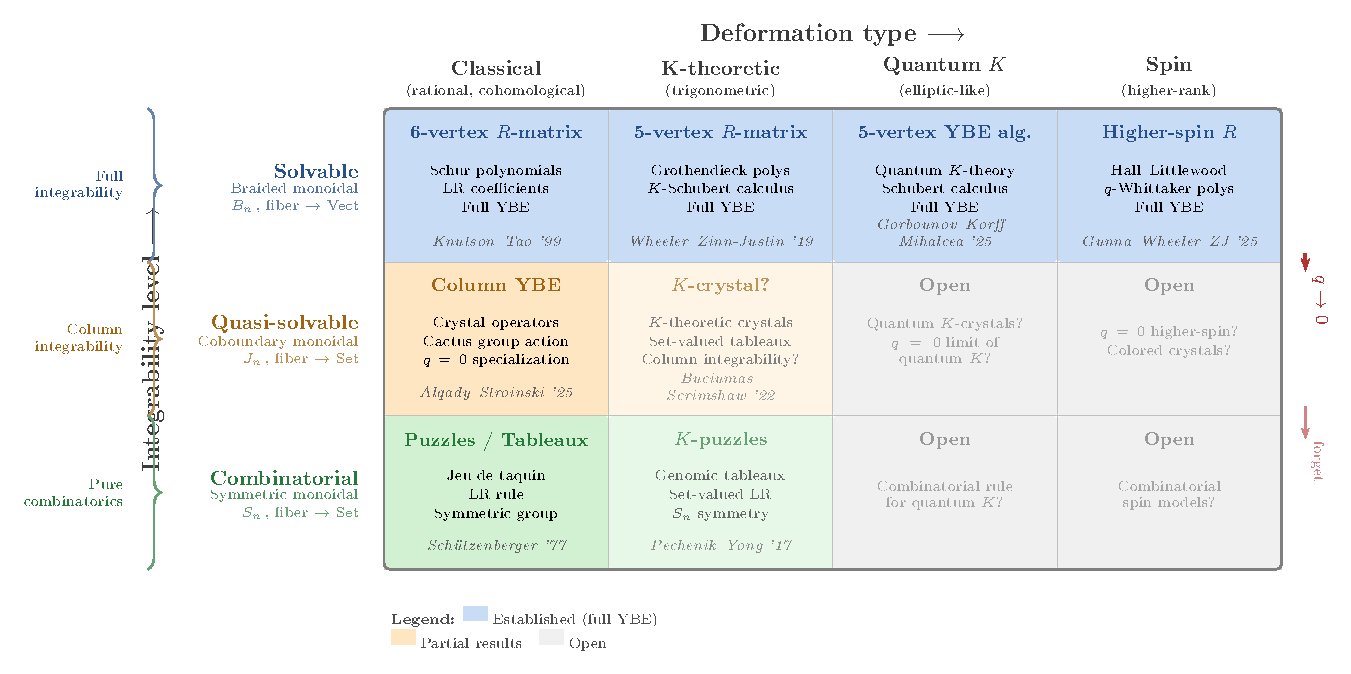
\includegraphics[width=\textwidth]{phase-diagram.pdf}
\caption{The categorical phase diagram.  The vertical axis parameterises
the integrability level (equivalently, the monoidal category type);
the horizontal axis parameterises the deformation type.  Filled cells
have established lattice models; lightly shaded cells have partial
results; empty cells are open.  The downward arrows indicate the
forgetful functors governed by the Hecke chain
$H_q \to H_0 \to \mathbb{C}[S_k]$.}
\label{fig:phase-diagram}
\end{figure}

\subsubsection*{A third dimension?}

The Tikhonov invariant $\kappa = (1-qp)/(1-p)$ suggests that the
phase diagram may have more structure than a flat grid.
The M\"obius formula~\eqref{eq:mobius} foliates the $(p,q)$ plane
into curves of constant $\kappa$: each curve represents a one-parameter
family of $(p,q)$ values producing the same asymptotic behaviour.  The
cactus locus --- the set of $(p,q)$ values where the cactus generator
emerges at $p = 1/2$ --- traces the line $\kappa = 2 - q$, a
constraint relating the interpolation and deformation parameters.

\begin{question}
Is the M\"obius action on $(p,q)$ related to the $\mathrm{PGL}(2)$
action on spectral parameters (Remark~\ref{rem:pgl2})?  If so, $\kappa$
would serve as a coordinate on a third axis --- the \emph{transition depth}
between integrability levels --- and the phase diagram would live on a surface
rather than a plane, with vertical transitions mediated by a continuous invariant.
One can test this by computing R-matrix eigenvalues and the Tikhonov invariant
$\kappa$ for small examples and checking whether they transform under the same
$\mathrm{PGL}(2)$.
\end{question}

\subsubsection*{What the diagram explains}

We close by returning to the question that opened the paper: why do so
many independent combinatorial models for LR coefficients exist?

The phase diagram provides an answer at two levels.  \emph{Horizontally},
models proliferate because the Yang-Baxter equation generates the
Yang-Baxter groupoid (Section~\ref{sec:groupoid-bn}): every R-matrix
move produces a new model computing the same coefficient.  The groupoid
is rich because the YBE has many solutions and many symmetries; the
bijections between models are morphisms, not miracles.
\emph{Vertically}, models proliferate because the categorical hierarchy
provides multiple projections of the same structure: the braided level
sees the spectral parameter, the coboundary level sees the multiplicity
bundle, and the symmetric level sees only the bare coefficient.  Each
level has its own characters, its own symmetry group, its own notion
of integrability --- and each level casts its own combinatorial
shadow.

The coefficients themselves --- $c^\nu_{\lambda,\mu}$, those
nonnegative integers governing the multiplication of Schur functions
--- sit at the intersection of all projections.  They are the invariant
that every level computes, every model records, and every forgetful
functor preserves.  The multiplicity of descriptions is not a defect
of the theory but a reflection of its depth: the same integers, seen
from above through a spectral parameter, from the middle through a
multiplicity bundle, and from below through a crystal basis, look
different at each level but agree on the count.  The phase diagram
is the map that says which view you are taking and what you have
chosen not to see.


\end{document}
